\documentclass{article}
\usepackage[titletoc, title, toc]{appendix}
\usepackage{hyperref}
\usepackage{graphicx}

\begin{document}
\title{System Design Document for NeedForSpeed (SDD)}
\author{}
\date{}
\maketitle

\tableofcontents

\noindent
\\
\\
\textbf{Version}: 1.0 \\
\textbf{Date}: \today \\
\textbf{Authors}: Anton \\
This version overrides all previous versions.

\section{Introduction}
\subsection{Desgin goals}
The design must be modular to have to possibility to switch GUI ..

\subsection{Definitions, acronyms and abbreviations}
\begin{itemize}
  \item GUI, Graphical User Interface
  \item Java, platform independent programming language.
  \item MVC, a way to partition an application with a GUI into distinct parts avoiding
  mixing GUI-code and application code.
  \item JSON, fileformat used for transmitting data in a structured way.
  \item Android, mobile operating system. 
  \item libGDX, framework for developing games in Java.
\end{itemize}

\section{System Design}
\subsection{Overview}
The application uses a modified version of the MVC pattern for Android.

\subsubsection{Model Functionality}
The entry point to the model is the World class. We split the model into diffrent classes such as Player, Enemy etc.

\subsubsection{Global lookups}
We keep track of the game state with a global variable.

\subsubsection{Event handling}
Event handling for the game is put in the PlayerController class. Event handling for menus and back-key is handled by their respective Screen class.

\subsection{Software decomposition}
\subsubsection{General}
INSERT PACKAGE DIAGRAM etc.. \\
The application is decomposed into two main packages, android and core, this is required by libGDX. the android package is for android specific code and in the core package the application code.

The core package is futher decomposed into:
\begin{itemize}
  \item view, the GUI part of the application.
  \item screen, the GUI part of the application.
  \item controller, the controller classes for MVC.
  \item parallax, for parallax background.
  \item highscore, highscore module for reading / writing highscore from file.
  \item gamestate, keeps track of the game state.
  \item model, game logic for the application, model part of MVC.
\end{itemize}

There is also a package for testing (should this be here??)

\subsubsection{Decomposition into subsystem}
The only subsystem present are parallax and highscore.

\subsubsection{Layering}
see figure \ref{fig:stan}

\subsubsection{Dependency analysis}
see figure \ref{fig:stan}


\begin{figure}[h]
  \centering
  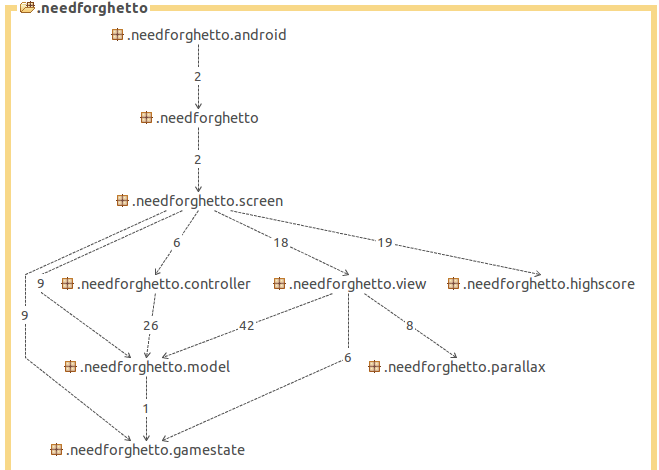
\includegraphics[width=0.8\textwidth]{stan.png}
  \caption{Layering and Dependency analysis}
  \label{fig:stan}
\end{figure}

\subsection{Concurrency issues}
All concurrency is abstracted by libGDX. But interally libGDX renders on a separate thread(is this needed? is this even true, probably...).

\subsection{Persistent data management}
Assets (add to definitions ?) ,such as textures, are persistent and operated on with functions provided by libGDX. Highscore data is handled through the preferences (add to definitions?) interface. 

Level design data is stored as JSON files.

\subsection{Access control and security}
NA


\subsection{Boundary conditions}
The application is launched and exited as a normal android application.

\section{References}
\begin{enumerate}
  \item ref1
  \item ref2
  \item ...
\end{enumerate}

\newpage
\begin{appendices}
  \section{Class diagrams}
  \section{Other stuff}
\end{appendices}

\end{document}